\documentclass{article}
\usepackage{ctex}
\usepackage{makecell}
\usepackage{graphicx}
\usepackage{geometry}
\usepackage{multirow}
\usepackage{multicol}
\usepackage{fancyhdr}
\usepackage{longtable}
\usepackage{color}
\usepackage{float}
\usepackage{listings}
\usepackage{xcolor}
\usepackage{hyperref}
\usepackage{footnote}
\usepackage{paralist}
\usepackage{amsmath}
\usepackage{subcaption}

\newcommand{\tabitem}{~~\llap{\textbullet}~~}
\renewcommand{\labelitemii}{\textbullet}
\renewcommand{\labelitemiii}{\textbullet}

\let\itemize\compactitem
\let\enditemize\endcompactitem
\let\enumerate\compactenum
\let\endenumerate\endcompactenum
\let\description\compactdesc
\let\enddescription\endcompactdesc

\geometry{a4paper,left=25mm,right=20mm,top=25mm,bottom=25mm}

\title{数字图像处理实验七}
\author{09021227~金桥}
\date{\today}

\lstset{
    numbers=left,
    keywordstyle= \color{ blue!70},
    commentstyle= \color{red!50!green!50!blue!50},
    rulesepcolor= \color{ red!20!green!20!blue!20} ,
    % escapeinside=``,
    numberstyle=\tt,
    numbersep=0em,
    xleftmargin=2em,
    breaklines,
    aboveskip=1em,
    framexleftmargin=2em,
    frame=shadowbox,
    basicstyle=\tt,
    language=C++
}

\begin{document}

\maketitle

\section{实验目标}


\begin{enumerate}
    \item 实验图像两幅自定义格式的医学 DR 图像,图像为RAW格式,都要进行图像细节处理。
    \item 自主设计或选择增强图像细节的算法,要求该算法适应原图像的灰度动态范围。算法设计时需要充分考虑图像的噪声放大问题,力求结果图像没有明显的噪声放大。图像细节增强算法全自动运行(尽可能针对不同图像人工调整参数)。 
    \item 程序使用 C++语言编写,增强算法必须自行编写程序实现,不允许使用OpenCV 等第三方库。 报告中体现对图像细节增强算法的思考
\end{enumerate}

\section{过程与方法}

\subsection{读取RAW格式图像}

根据图像格式,灰度有效范围为$[0, 4095]$, 为12位有效灰度,每像素两字节(最高4位数据无效,有效灰度保存于低12位)。数据文件为自定义格式(非标准格式)。

文件开始的4字节存放图像宽参数,其后4字节存放图像高参数,此两参数均为无符号长整型(\texttt{unsigned long}),紧随其后为按光栅扫描顺序(从左向右,逐行扫描)存放的像素值,像素值为无符号短整型(\texttt{unsigned short})。所有多字节数据都按Intel顺序(即低字节在前,高字节在后)存放,文件不包含其它数据。

根据描述,编写了对应的读取函数 \texttt{readFromRaw},按照给定格式进行读取并将像素压缩至8位深度,即$[0, 255]$。

\subsection{图像增强算法}

采用CLAHE算法进行增强,由于自行编写的CLAHE在精度上比起OpenCV实现略差,因此采取3次CLAHE算法增强。


CLAHE计算过程如下,具体实现参见代码。

\begin{itemize}
    \item 首先将图像分块(OpenCV默认$8\times 8$分块, 与其保持一致),图像边缘不够的进行补齐
    \item 对每个分块进行处理:
    \begin{itemize}
        \item 计算出分块的直方图数值
        \item 根据预设的阈值对直方图进行裁切,将高处的部分均匀补齐至所有灰度上
        \item 返回处理后的直方图
    \end{itemize}
    \item 为防止棋盘效应对图像造成割裂,采用双线性插值
    \begin{itemize}
        \item 对每个块的像素,取离它最近的四个分块,并取出四个分块处理后对应的灰度值
        \item 假设从上到下,从左到右,四个灰度值分别是 $r_1, r_2, r_3, r_4$
        \item 假设在离这个像素最近的四个分块的中心点形成的矩形中:
        \begin{itemize}
            \item 这个像素距离上下边界的距离是 $y_1, y_2$,左右边界距离 $x_1, x_2$,分块横纵大小 $w, h$
        \end{itemize}
        \item 代入下式计算最终像素灰度$r$:$$r = (r_1 \frac{x_1}{w} + r_2 \frac{x_2}{w})\frac{y_1}{h} + (r_3 \frac{x_1}{w} + r_4 \frac{x_2}{w})\frac{y_2}{h}$$
    \end{itemize}
\end{itemize}

\section{结果}

\begin{figure}[H]
    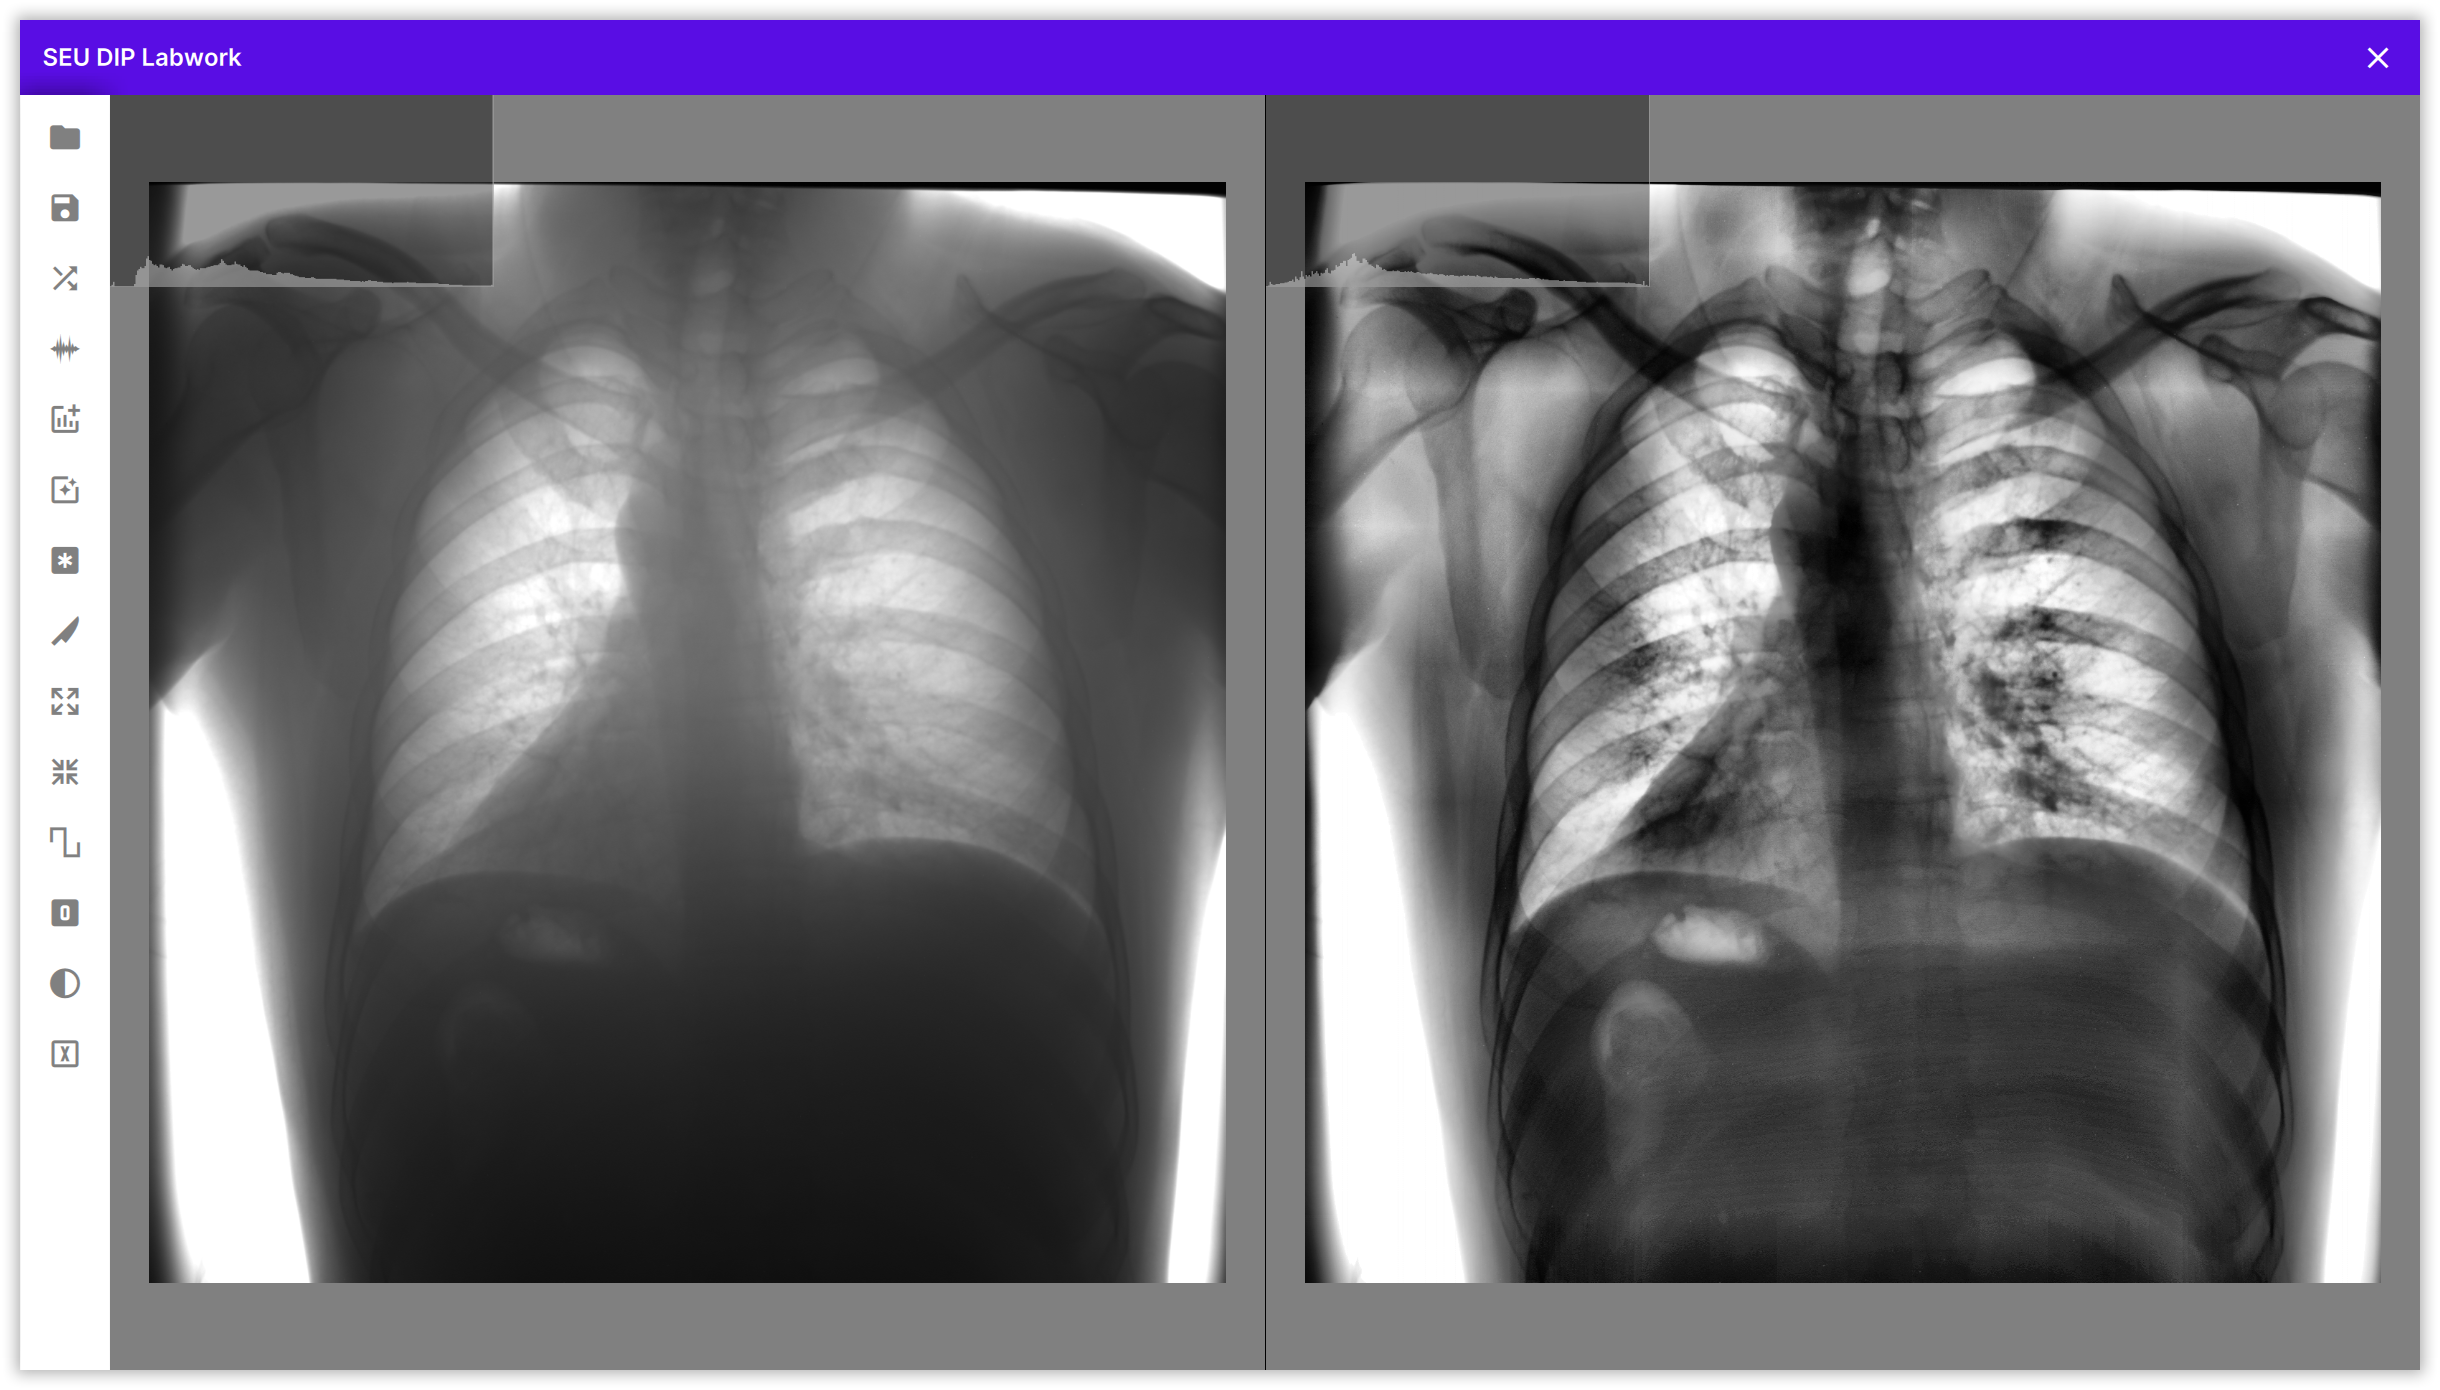
\includegraphics[width=\textwidth]{img/lung.png}
\end{figure}

\begin{figure}[H]
    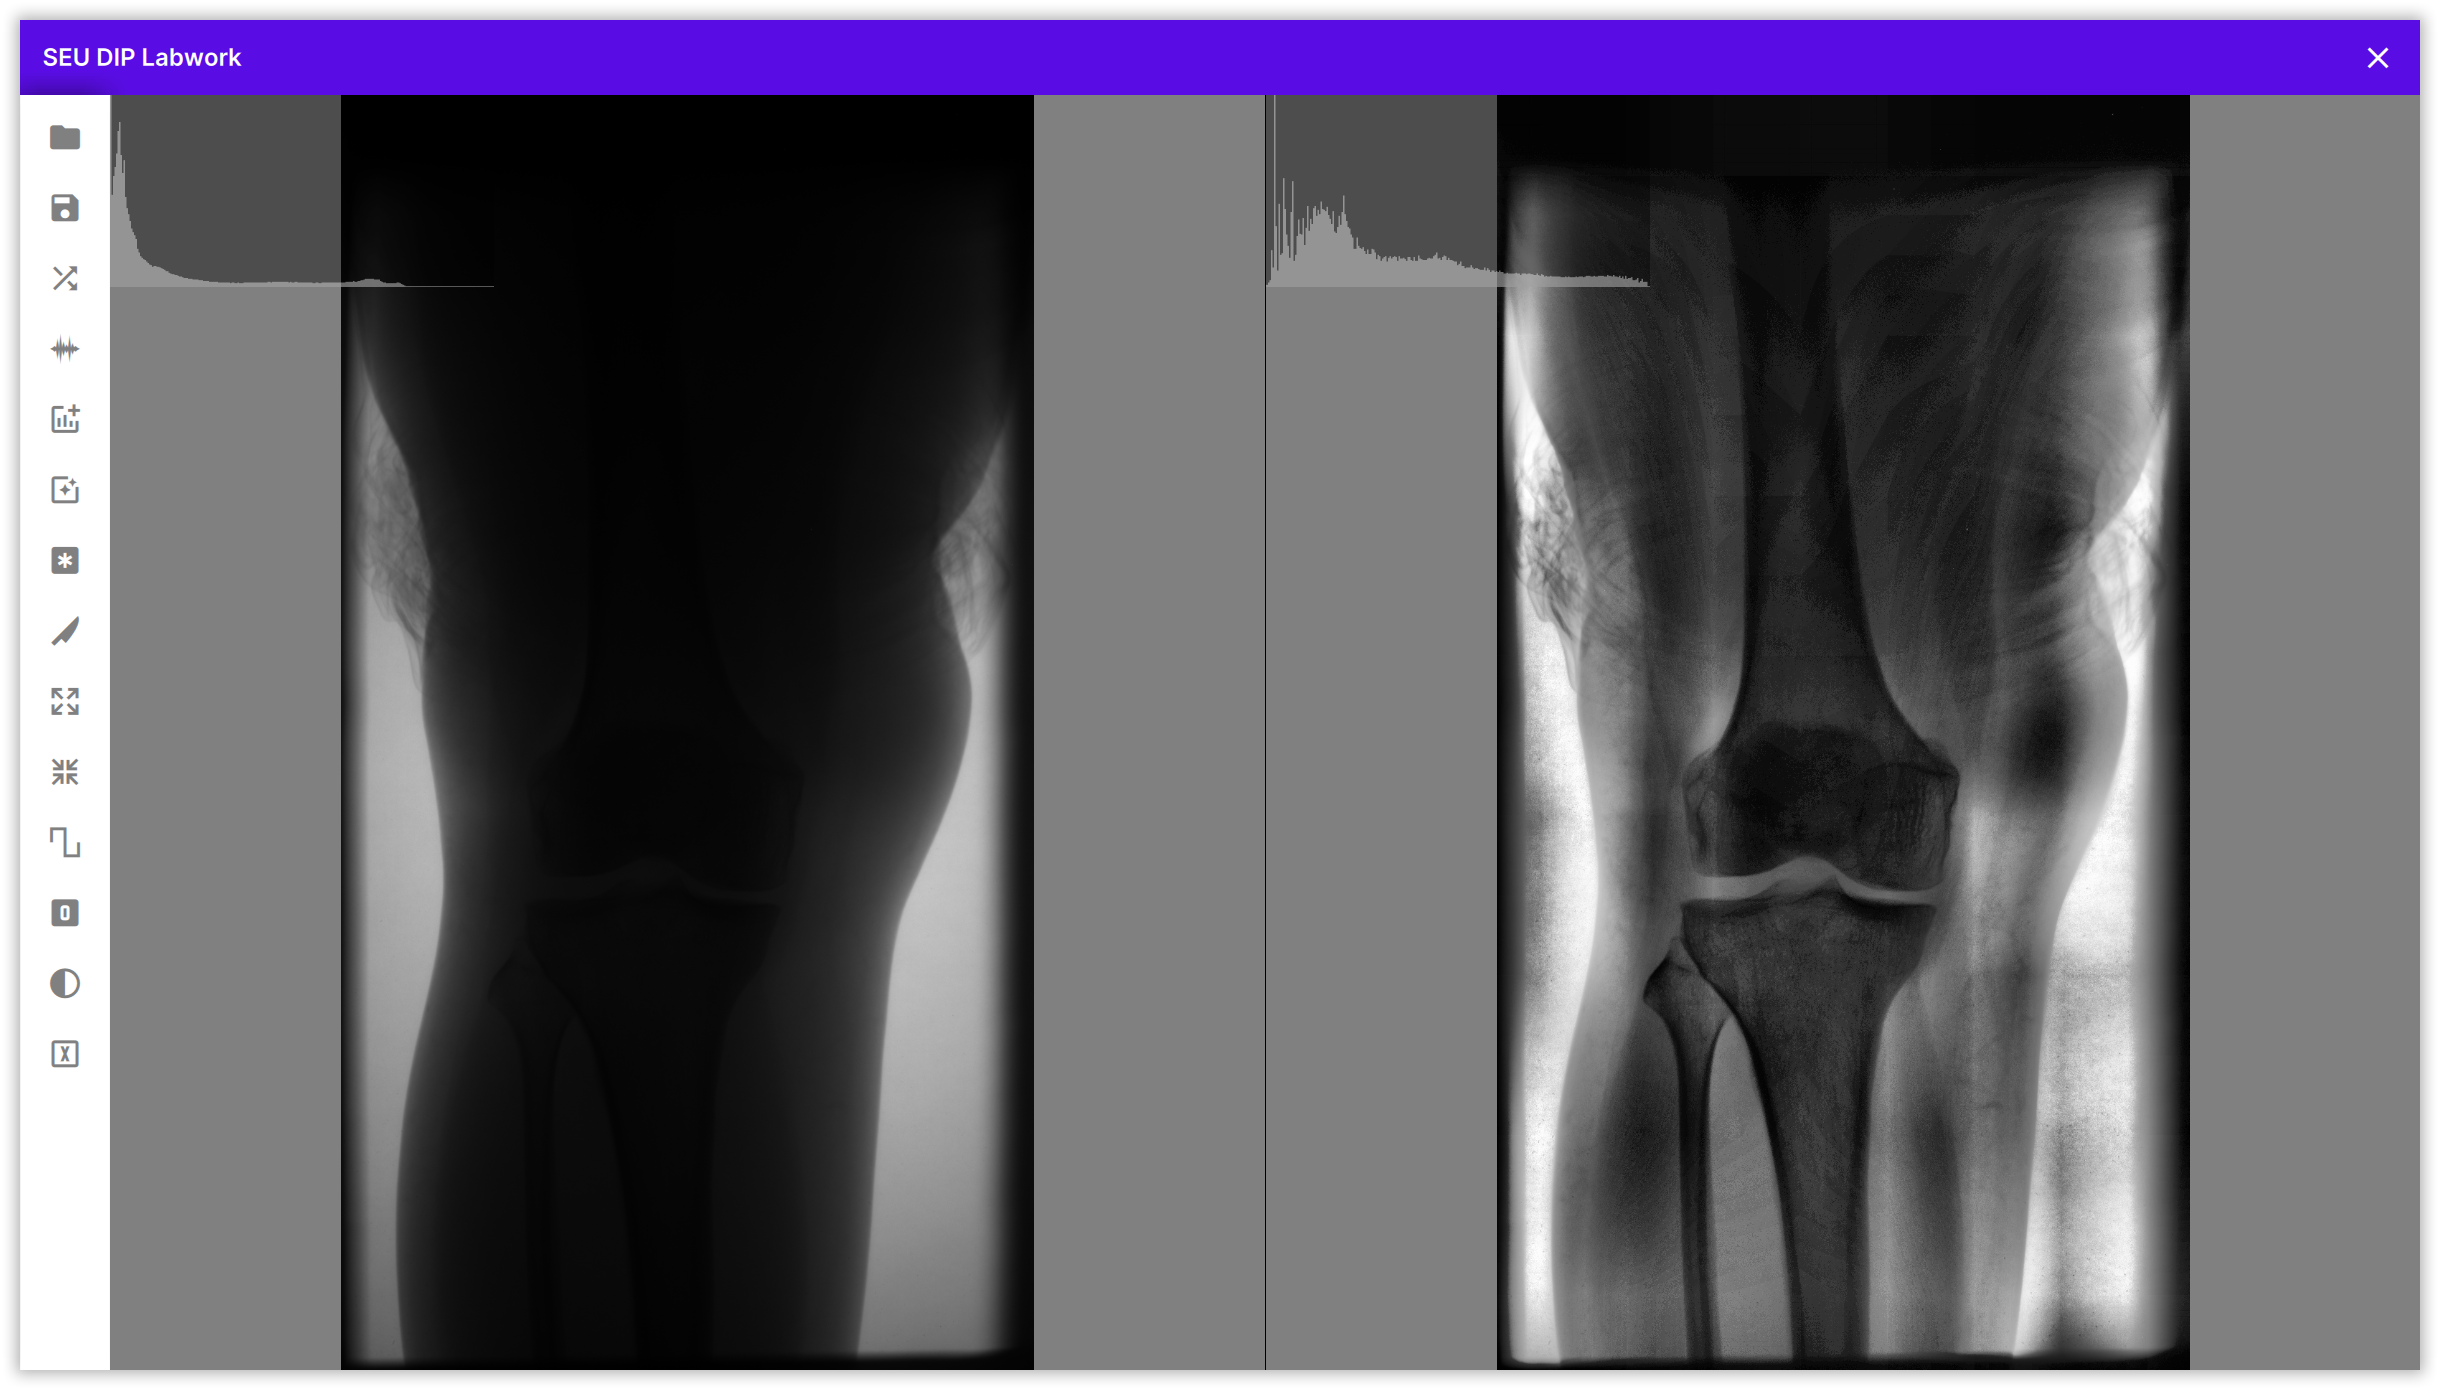
\includegraphics[width=\textwidth]{img/knee.png}
\end{figure}

\end{document}
